\documentclass[12pt]{article}
\usepackage[a4paper, left=2cm, right=2cm, top=2cm, bottom=2cm]{geometry}
\usepackage{fontspec}
\usepackage{booktabs}
\usepackage{amsmath, amsfonts}
\usepackage{graphicx}
\usepackage{polyglossia}
\usepackage{float}
\setdefaultlanguage{greek}
\setotherlanguage{english}
\setmainfont{Palatino Linotype}
\newfontfamily\greekfonttt{Liberation Mono}[Scale=MatchLowercase]
%\setmonofont{Latin Modern Mono}[Scale=MatchLowercase]
\usepackage{subcaption}
\usepackage{siunitx}
\usepackage{bm}

% This is for code
\usepackage{listings}
\usepackage{xcolor} % Required for custom colors

% This is for CSV
\usepackage{csvsimple-l3}


% Define custom colors
\definecolor{codegreen}{rgb}{0,0.6,0}
\definecolor{codegray}{rgb}{0.5,0.5,0.5}
\definecolor{codepurple}{rgb}{0.58,0,0.82}
\definecolor{backcolour}{rgb}{0.95,0.95,0.92}

% Define a custom style for C code
\lstdefinestyle{CStyle}{
    language=C,
    backgroundcolor=\color{backcolour},   
    commentstyle=\color{codegreen},
    keywordstyle=\color{blue}\bfseries,
    numberstyle=\tiny\color{codegray},
    stringstyle=\color{codepurple},
    basicstyle=\ttfamily\scriptsize,
    breakatwhitespace=false,         
    breaklines=true,                 
    captionpos=b,                    
    keepspaces=true,                 
    numbers=left,                    
    numbersep=5pt,                  
    showspaces=false,                
    showstringspaces=false,
    showtabs=false,                  
    tabsize=4
}

% Define a custom style for Makefile
\lstdefinestyle{MakeStyle}{
    language=make,
    backgroundcolor=\color{backcolour},
    commentstyle=\color{codegreen},
    keywordstyle=\color{blue}\bfseries,
    numberstyle=\tiny\color{codegray},
    stringstyle=\color{codepurple},
    basicstyle=\ttfamily\scriptsize,
    breakatwhitespace=false,
    breaklines=true,
    captionpos=b,
    keepspaces=true,
    numbers=left,
    numbersep=5pt,
    showspaces=false,
    showstringspaces=false,
    showtabs=false,
    tabsize=4
}

% Define a custom style for Bash
\lstdefinestyle{BashStyle}{
    language=bash,
    backgroundcolor=\color{backcolour},
    commentstyle=\color{codegreen},
    keywordstyle=\color{blue}\bfseries,
    numberstyle=\tiny\color{codegray},
    stringstyle=\color{codepurple},
    basicstyle=\ttfamily\footnotesize,
    breakatwhitespace=false,
    breaklines=true,
    captionpos=b,
    keepspaces=true,
    numbers=left,
    numbersep=5pt,
    showspaces=false,
    showstringspaces=false,
    showtabs=false,
    tabsize=4
}

% Define ARM Assembly language for listings
\lstdefinelanguage{ARM}{
    morekeywords=[1]{% Data processing & arithmetic
        mov, mvn, add, adc, sub, sbc, rsb, rsc,
        mul, mla, umull, umlal, smull, smlal,
        and, orr, eor, bic, lsl, lsr, asr, ror, rrx,
        cmp, cmn, tst, teq,
        % Memory access & stack
        ldr, ldrb, ldrh, ldrsb, ldrsh, ldrex, ldm, ldmia, ldmfd,
        str, strb, strh, strex, stm, stmia, stmfd,
        push, pop, swp, swpb,
        % Branching & system
        b, bl, bx, blx, swi, svc, nop,
        % Common conditional suffixes
        beq, bne, bcs, bhs, bcc, blo, bmi, bpl, bvs, bvc, bhi, bls, bge, blt, bgt, ble,
        moveq, movne, movhs, movlo, movhi, movls, movge, movlt, movgt, movle,
        addeq, addne, addhi, addlo, subeq, subne, subhi, sublo,
        bxeq, bxne
    },
    morekeywords=[2]{% Registers & assembler directives
        r0, r1, r2, r3, r4, r5, r6, r7, r8, r9, r10, r11, r12, r13, r14, r15,
        sp, lr, pc, cpsr, spsr,
        .text, .data, .bss, .rodata, .section,
        .global, .globl, .extern, .type, .size,
        .align, .balign, .p2align,
        .byte, .hword, .short, .word, .long, .quad, .float, .double,
        .ascii, .asciz, .string, .space, .skip, .zero, .equ, .set,
        .arm, .thumb, .thumb_func, .syntax, .arch, .cpu, .fpu, .end
    },
    sensitive=false,
    morecomment=[l]{@},
    morecomment=[l]{//},
    morecomment=[s]{/*}{*/},
    morestring=[b]",
    morestring=[b]'
}

% Define a custom style for ARM Assembly matching CStyle
\lstdefinestyle{ARMStyle}{
    language=ARM,
    backgroundcolor=\color{backcolour},
    commentstyle=\color{codegreen},
    keywordstyle=\color{blue}\bfseries,
    keywordstyle=[2]\color{teal}\bfseries,
    numberstyle=\tiny\color{codegray},
    stringstyle=\color{codepurple},
    basicstyle=\ttfamily\scriptsize,
    breakatwhitespace=false,
    breaklines=true,
    captionpos=b,
    keepspaces=true,
    numbers=left,
    numbersep=5pt,
    showspaces=false,
    showstringspaces=false,
    showtabs=false,
    tabsize=4,
    alsoletter={.}
}

\begin{document}

% --- HEADER START ---
\noindent
\begin{minipage}[t]{\textwidth}
    {\large \textbf{Εθνικό Μετσόβιο Πολυτεχνείο}} \\
    \textbf{Σχολή Ηλεκτρολόγων Μηχανικών και Μηχανικών Υπολογιστών} \\    
    \textbf{Τομέας Τεχνολογίας Πληροφορικής και Υπολογιστών} \\
    Μάθημα: "Σχεδιασμός Ενσωματωμένων Συστημάτων" \\
    Ακαδ. Έτος: 2026-2027
\end{minipage}

\vspace{0.2cm}
\hrule height 1pt
\vspace{1cm}
% --- HEADER END ---


% --- TITLE SECTION ---
\begin{center}
    {\LARGE \textbf{3η Εργαστηριακή Άσκηση}} \\[0.5cm]
    {\large Εργασία σε Assembly του Επεξεργαστή ARM}
\end{center}
\vspace{1cm}


% --- AUTHORS SECTION ---
\begin{center}
	\textbf{Αποστολόπουλος Νικόλαος} \\
	(03122614) \\
	\textbf{Γκριμπογιάννης Χαρίλαος} \\
	(03122002)
\end{center}
\vspace{1cm}

% --- ABSTRACT SECTION ---
\begin{center}
    \textbf{\large Περίληψη}
\end{center}

\noindent
Η παρούσα εργασία υλοποιήθηκε στα πλαίσια του μαθήματος "Σχεδιασμός Ενσωματωμένων Συστημάτων" και αφορά στην εξοικείωση με τον προγραμματισμό σε Assembly του επεξεργαστή ARM και στη σύνδεση Assembly και γλώσσας C.
\pagebreak

\tableofcontents
\pagebreak

\section{Μετατροπή Εισόδου από Τερματικό}
Γράφουμε ένα πρόγραμμα σε assembly του επεξεργαστή ARM, το οποίο λαμβάνει ως είσοδο από το τερματικό μια συμβολοσειρά μεγέθους έως 32 χαρακτήρες. Αν δοθούν περισσότεροι χαρακτήρες, τότε αυτοί αγνοούνται. Το πρόγραμμα εκτελεί την ακόλουθη μετατροπή:
\begin{itemize}
\item Αν ο χαρακτήρας είναι κεφαλαίο γράμμα της αγγλικής αλφαβήτου, τότε μετατρέπεται σε πεζό και αντίστροφα ('A'-'Z' $\leftrightarrow$ 'a'-'z').
\item Αν ο χαρακτήρας είναι δεκαδικό ψηφίο, τότε εκτελείται η μετατροπή '0'-'4' $\leftrightarrow$ '5'-'9'.
\item Οι υπόλοιποι χαρακτήρες παραμένουν αμετάβλητοι.
\end{itemize}
Το πρόγραμμα είναι συνεχούς λειτουργίας και τερματίζει όταν λάβει ως είσοδο συμβολοσειρά μήκους 1 που αποτελείται από τον χαρακτήρα 'Q' ή 'q'.

Στην υλοποίησή μας χρησιμοποιούμε συναρτήσεις της βιβλιοθήκης της C (scanf, printf, getchar) και αξιοποιούμε τον κώδικα ASCII ώστε μέσω αριθμητικών συγκρίσεων και πράξεων να εφαρμόζεται ο παραπάνω μετασχηματισμός στους χαρακτήρες της συμβολοσειράς. Η μετατροπή από πεζό σε κεφαλαίο και αντίστροφα γίνεται με ένα μόνο bit flip, ενώ η μετατροπή των δεκαδικών ψηφίων γίνεται με modulo πρόσθεση.

\lstinputlisting[style=ARMStyle, caption={Κώδικας ARM Assembly (Ερώτημα 1)}, label={lst:transform}]{transform.s}

\begin{figure} [H]
\centering
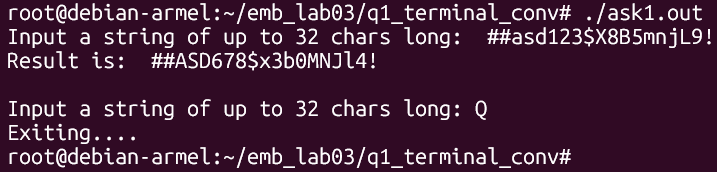
\includegraphics[width=0.8\linewidth]{q1_res}
\caption{Ενδεικτική εκτέλεση του προγράμματος}
\label{fig:q1-res}
\end{figure}

\section{Επικοινωνία των guest και host Μηχανημάτων μέσω Σειριακής Θύρας}
Στην παρούσα παράγραφο δημιουργούμε δύο προγράμματα, ένα πρόγραμμα C το οποίο τρέχει στο host μηχάνημα και ένα πρόγραμμα ARM Assembly το οποίο τρέχει στο guest μηχάνημα. Το πρόγραμμα του host μηχανήματος δέχεται ως είσοδο μια συμβολοσειρά μήκους έως 64 χαρακτήρες, αποστέλλει αυτή τη συμβολοσειρά μέσω σειριακής θύρας στο guest μηχάνημα, το οποίο με τη σειρά του απαντάει ποιος είναι ο πιο συχνά εμφανιζόμενος χαρακτήρας της συμβολοσειράς (εξαιρείται το space - ASCII 32) και πόσες φορές εμφανίζεται. Εφόσον δύο ή περισσότεροι χαρακτήρες έχουν τη μέγιστη συχνότητα εμφάνισης, επιλέγεται ο χαρακτήρας με τον μικρότερο κωδικό ASCII.

Για την επικοινωνία host - guest επιλέξαμε το πρόγραμμα του host να ανοίγει το /dev/ptmx σύμφωνα με τις οδηγίες που δίνονται στο man pts, να τυπώνει στο τερματικό το αρχείο /dev/pts/N που δημιουργήθηκε και ύστερα να περιμένει έως ότου δώσουμε σαν όρισμα στο qemu αυτό το αρχείο με το -serial option. Αφού κάνει boot το Debian ARM στο qemu, τρέχουμε το guest πρόγραμμα και επιστρέφουμε στο τερματικό του host, πατάμε Enter και ξεκινάει η κανονική λειτουργία, κατά την οποία ο host στέλνει στον guest τις συμβολοσειρές που ο χρήστης πληκτρολογεί στο τερματικό, ο guest τις επεξεργάζεται και στέλνει πίσω στον host το πιο σύνηθες σύμβολο και το πλήθος των εμφανίσεών του για να τα τυπώσει ο host στο τερματικό.

Σημειώνουμε ότι η υλοποίησή μας προϋποθέτει να στέλνονται μόνο συμβολοσειρές τερματισμένες με '\textbackslash n'.

\lstinputlisting[style=CStyle, caption={Κώδικας C - host (Ερώτημα 2)}, label={lst:q2-host}]{host_comm.c}

Για το πρόγραμμα του guest σκεφτήκαμε δύο υλοποιήσεις. Η πρώτη βασίζεται σε 95 μετρητές που αποθηκεύουν το πλήθος των εμφανίσεων κάθε printable ASCII χαρακτήρα, ενώ η δεύτερη μετράει τις εμφανίσεις κάθε χαρακτήρα που βρίσκεται στη συμβολοσειρά, χρησιμοποιώντας εμφωλευμένο βρόχο. Προφανώς, η πρώτη υλοποίηση εκτελείται ταχύτερα, αλλά έχει το μειονέκτημα ότι δεσμεύει αρκετή μνήμη. Λαμβάνοντας υπόψη το γεγονός ότι η σειριακή επικοινωνία αποτελεί το bottleneck όσον αφορά την ταχύτητα, επιλέξαμε τη δεύτερη υλοποίηση ούτως ώστε να ελαχιστοποιήσουμε το αποτύπωμα στη μνήμη.

\lstinputlisting[style=ARMStyle, caption={Κώδικας ARM Assembly - guest (Ερώτημα 2)}, label={lst:q2-guest}]{guest_freq.s}

Σημειώνουμε ότι έχουμε διατηρήσει το prompt "Please give a string to send to host:" καθώς αυτό εμφανίζεται στην εκφώνηση της Άσκησης, παρά το γεγονός ότι η συμβολοσειρά αποστέλλεται στον guest και όχι στον host. Ενδεικτικά παραθέτουμε το παρακάτω παράδειγμα εκτέλεσης.

\begin{figure} [H]
\centering
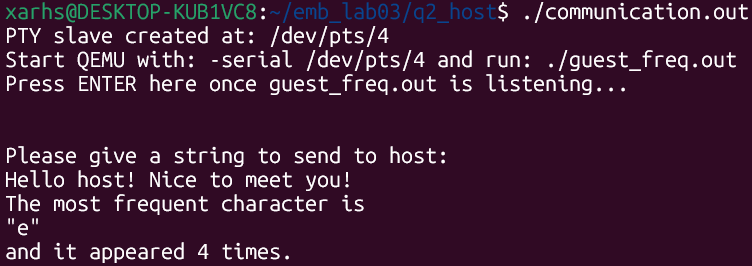
\includegraphics[width=0.8\linewidth]{q2_res}
\caption{Εκτέλεση του προγράμματος του host}
\label{fig:q2-host}
\end{figure}

\section{Σύνδεση Κώδικα C με Κώδικα Assembly του Επεξεργαστή ARM}
Στην παρούσα παράγραφο αντικαθιστούμε τις συναρτήσεις strlen, strcpy, strcat και strcmp της βιβλιοθήκης string.h με δικές μας συναρτήσεις γραμμένες σε ARM Assembly. Τις συναρτήσεις αυτές τις καλούμε (ως extern) στο πρόγραμμα C string\_manipulation.c, το οποίο ανοίγει ένα αρχείο 512 γραμμών, κάθε γραμμή του οποίου περιέχει μια τυχαία κατασκευασμένη συμβολοσειρά, μεγέθους 8 έως 64 χαρακτήρων. Το πρόγραμμα παράγει τρία αρχεία εξόδου:
\begin{enumerate}
\item Το πρώτο περιέχει το μήκος της κάθε γραμμής του αρχείου εισόδου.
\item Το δεύτερο περιέχει τις συμβολοσειρές του αρχείου εισόδου ενωμένες (concatenated) ανά 2.
\item Το τρίτο περιέχει τις συμβολοσειρές του αρχείου εισόδου ταξινομημένες σε αύξουσα αλφαβητική σειρά.
\end{enumerate}

Για να γράψουμε τις συναρτήσεις ώστε να διατηρείται η λειτουργικότητα των συναρτήσεων της string.h, συμβουλευόμαστε το Reference της C.

\lstinputlisting[style=ARMStyle, caption={ARM Assembly strlen  (Ερώτημα 3)}, label={lst:strlen}]{strlen.s}

\lstinputlisting[style=ARMStyle, caption={ARM Assembly strcpy  (Ερώτημα 3)}, label={lst:strcpy}]{strcpy.s}

\lstinputlisting[style=ARMStyle, caption={ARM Assembly strcat  (Ερώτημα 3)}, label={lst:strcat}]{strcat.s}

\lstinputlisting[style=ARMStyle, caption={ARM Assembly strcmp  (Ερώτημα 3)}, label={lst:strcmp}]{strcmp.s}

Για τη σωστή μεταγλώττιση και σύνδεση των επιμέρους αρχείων γράφουμε το ακόλουθο Makefile.

\lstinputlisting[style=MakeStyle, caption={Makefile  (Ερώτημα 3)}, label={lst:makefile}]{Makefile.txt}

Για να ελέγξουμε την ορθότητα της υλοποίησής μας γράφουμε ένα sh script ονόματι test\_q3.sh το οποίο εκτελούμε τρέχοντας τις εντολές:

\begin{lstlisting}[style=BashStyle]
sed -i 's/\r$//' test_q3.sh
chmod +x test_q3.sh
./test_q3.sh
\end{lstlisting}

Το script αυτό αξιοποιεί το Makefile, σιγουρεύει ότι οι συναρτήσεις έχουν αντικατασταθεί από τις δικές μας και τρέχει το πρόγραμμα string\_manipulation για τα δύο example input αρχεία. Ύστερα, ξανατρέχει το string\_manipulation με τις συναρτήσεις της C και ελέγχει αν τα παραγόμενα output αρχεία είναι ίδια. Στο ακόλουθο Σχήμα φαίνεται η εκτέλεση του script αυτού.

\begin{figure} [H]
\centering
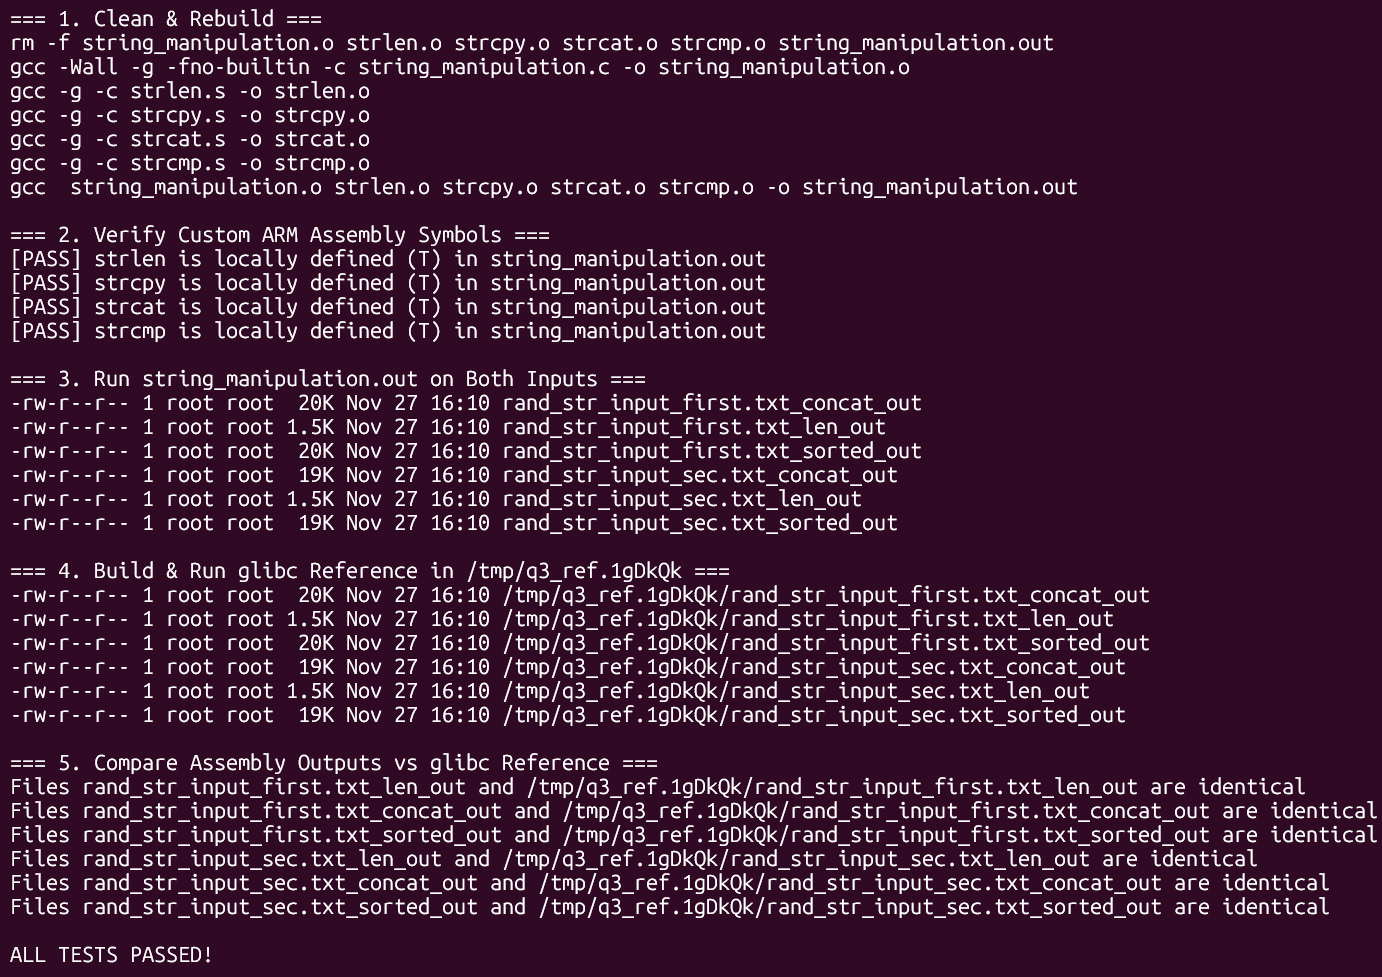
\includegraphics[width=0.8\linewidth]{q3_res}
\caption{Έλεγχος λειτουργικότητας των ARM Assembly συναρτήσεων}
\label{fig:q3-res}
\end{figure}

\end{document}
